\everymath{\displaystyle}
\documentclass{beamer}
% \documentclass[handout]{beamer}

%\usepackage[pdftex]{color,graphicx}
\usepackage{amsmath,amssymb,amsfonts}

\mode<presentation>
{
  % \usetheme{Darmstadt}
  % \usetheme[hideothersubsections]{Hannover}
  % \usetheme[hideothersubsections]{Goettingen}
  \usetheme[hideothersubsections, right]{Berkeley}

  \usecolortheme{seahorse}
  % \usecolortheme{dolphin}
  \usecolortheme{rose}
  % \usecolortheme{orchid}

  \useinnertheme[shadow]{rounded}

  \setbeamercovered{transparent}
  % or whatever (possibly just delete it)
}

\mode<handout>{
  \setbeamercolor{background canvas}{bg=black!5}
  \usepackage{pgfpages}
  \pgfpagesuselayout{4 on 1}[a4paper,border shrink=5mm, landscape]
}

\usepackage[brazilian]{babel}
% or whatever

% \usepackage[latin1]{inputenc}
\usepackage[utf8]{inputenc}
% or whatever

\usepackage{times}
%\usepackage[T1]{fontenc}
% Or whatever. Note that the encoding and the font should match. If T1
% does not look nice, try deleting the line with the fontenc.


\title%[] % (optional, use only with long paper titles)
{Tópicos de busca bibliográfica}

\subtitle
{Google-fu et al} % (optional)

\author%[] % (optional, use only with lots of authors)
{Felipe Figueiredo}% \and S.~Another\inst{2}}
% - Use the \inst{?} command only if the authors have different
%   affiliation.

\institute[INTO] % (optional, but mostly needed)
{Instituto Nacional de Traumatologia e Ortopedia
}
  % \inst{1}%
  % Department of Computer Science\\
  % University of Somewhere
  % \and
  % \inst{2}%
  % Department of Theoretical Philosophy\\
  % University of Elsewhere}
% - Use the \inst command only if there are several affiliations.
% - Keep it simple, no one is interested in your street address.

\date%[] % (optional)
{}

% \subject{Talks}
% This is only inserted into the PDF information catalog. Can be left
% out. 



% If you have a file called "university-logo-filename.xxx", where xxx
% is a graphic format that can be processed by latex or pdflatex,
% resp., then you can add a logo as follows:

\pgfdeclareimage[height=1.6cm]{university-logo}{../logo}
\logo{\pgfuseimage{university-logo}}



% Delete this, if you do not want the table of contents to pop up at
% the beginning of each subsection:
\AtBeginSubsection[]
%\AtBeginSection[]
{
  \begin{frame}<beamer>{Sumário}
    \tableofcontents[currentsection,currentsubsection]
  \end{frame}
}


% If you wish to uncover everything in a step-wise fashion, uncomment
% the following command: 

% \beamerdefaultoverlayspecification{<+->}


\begin{document}

\begin{frame}
  \titlepage
\end{frame}

\begin{frame}{Sumário}
  \tableofcontents
  % You might wish to add the option [pausesections]
\end{frame}


%% Template
% \section{}

% \subsection{}

% \begin{frame}{}
%   \begin{itemize}
%   \item 
%   \end{itemize}
% \end{frame}

% \begin{frame}
%   \begin{columns}
%     \begin{column}{5cm}
%     \end{column}
%     \begin{column}{5cm}
%     \end{column}
%   \end{columns}
% \end{frame}

% \begin{frame}{}
%   \includegraphics[height=0.4\textheight]{file1}
%   \includegraphics[height=0.4\textheight]{file2}
%   \includegraphics[height=0.4\textheight]{file3}
%   \begin{figure}
%     \caption{}
%   \end{figure}
% \end{frame}

% \begin{frame}{}
%   \begin{definition}
%   \end{definition}
%   \begin{example}
%   \end{example}
%   \begin{block}{Exercício}
%   \end{block}
% \end{frame}

\section{Discussão da aula passada}

% \subsection{Discussão da aula passada}

\begin{frame}{Discussão da aula passada}
  \begin{block}{}
    Discussão da leitura obrigatória da aula passada
  \end{block}
\end{frame}

\section{Bases bibliográficas}

\begin{frame}{Bases bibliográficas na Internet}
  \begin{itemize}
    \footnotesize
  \item Antigamente localizava-se livros e revistas por fichas
    \begin{center}
      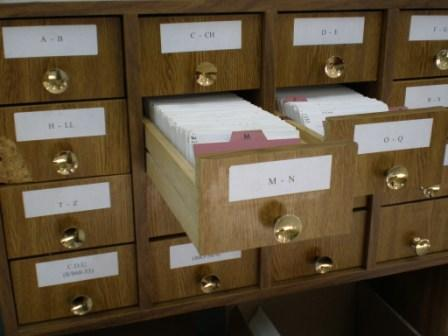
\includegraphics[height=.45\textheight]{Busca/fichas}
    \end{center}

  \item Hoje podemos fazer buscas profundas em bases bibliográficas
    (conteúdo completo das obras)
  \end{itemize}
\end{frame}

\begin{frame}{Exemplos}
  \begin{itemize}
    \footnotesize
  \item \alert{PUBMED} - \url{www.pubmed.org} (ou .com)
  \item \alert{PUBMED Central} - \url{www.ncbi.nlm.nih.gov/pmc/}
  \item \alert{Google Scholar} - \url{scholar.google.com}
  \item Web of Science - \url{www.webofknowledge.com}
  \item Scielo - \url{www.scielo.br}
  \item CrossRef - \url{www.crossref.org}
  \item etc\ldots
  \end{itemize}
\end{frame}

\subsection{PUBMED e PUBMED Central}

\begin{frame}{PUBMED}
  \begin{itemize}
    \footnotesize
  \item \alert{Mecanismo de busca}, mantido pelo governo dos EUA
    (NLM\footnote{National Library of Medicine} e
    NIH\footnote{National Institutes of Health})
  \item Acessa primariamente a base MEDLINE, entre outras
  \item Referências dos artigos são indexadas e catalogadas para busca
  \item Links para o conteúdo dos artigos (externos)
  \item Sugere artigos similares
  \item Exporta referências para gerenciadores bibliográficos
    (Mendeley, EndNote, etc)
  \end{itemize}
\end{frame}

\begin{frame}{MEDLINE}
  \begin{block}{Definição}
    Base bibliográfica de acesso gratuito de referências de Ciências
    da Saúde e afins
  \end{block}
  Disponíveis:
  \begin{itemize}
    \footnotesize
  \item Índice
  \item Abstract
  \item Link para artigo completo (em geral, site da editora)
  \end{itemize}
\end{frame}

\begin{frame}{MEDLINE (escopo)}
  \begin{block}{De acordo com a Wikipédia}
    \footnotesize
    Disciplinas: Medicine, nursing, pharmacy, dentistry, veterinary
    medicine, health care, biology, biochemistry, molecular evolution,
    biomedicine, history of medicine, health services research, AIDS,
    toxicology and environmental health, molecular biology,
    complementary medicine, behavioral sciences, chemical sciences,
    bioengineering, health policy development, environmental science,
    marine biology, plant and animal science, biophysics
  \end{block}
\end{frame}

\begin{frame}{PUBMED Central (PMC)}
  \begin{block}{Definição}
    Repositório gratuito de artigos Open-Access
  \end{block}
  Disponíveis:
  \begin{itemize}
    \footnotesize
  \item Índice
  \item Abstract
  \item Conteúdo integral
  \end{itemize}
\end{frame}

\begin{frame}{PUBMED Busca}
  \centering
  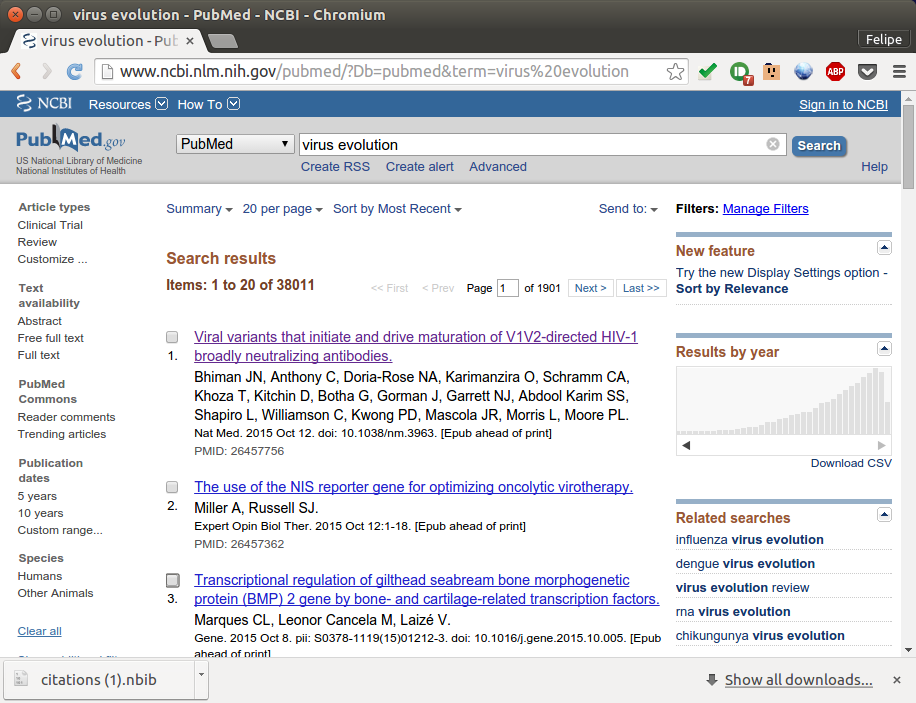
\includegraphics[height=.85\textheight]{Busca/pubmed-busca}
\end{frame}

\begin{frame}{PUBMED Artigo}
  \centering
  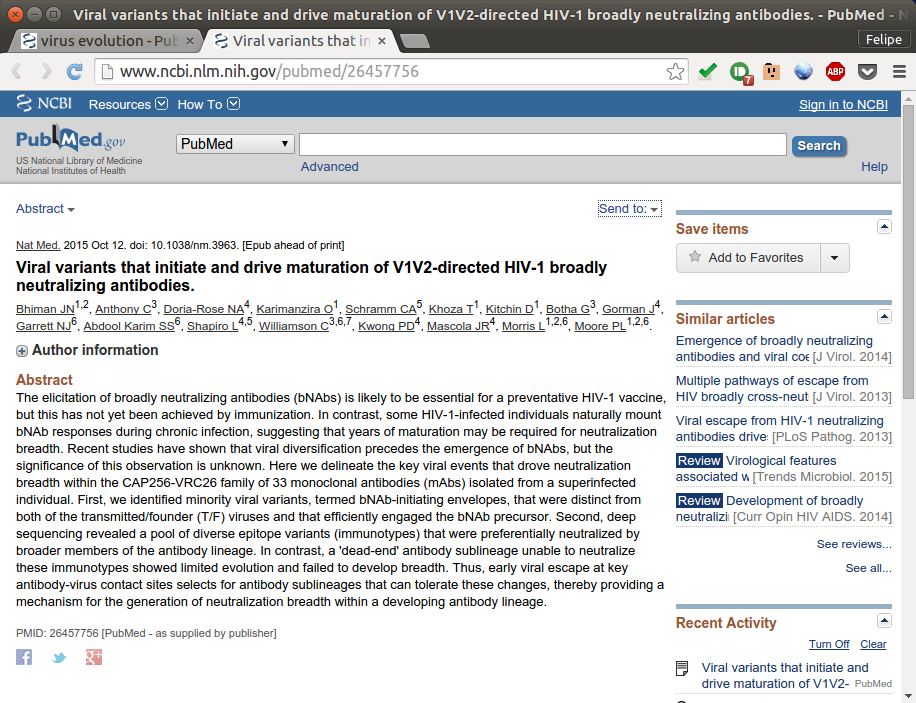
\includegraphics[height=.85\textheight]{Busca/pubmed-paper}
\end{frame}

\begin{frame}{PUBMED Exportando a referência}
  \centering
  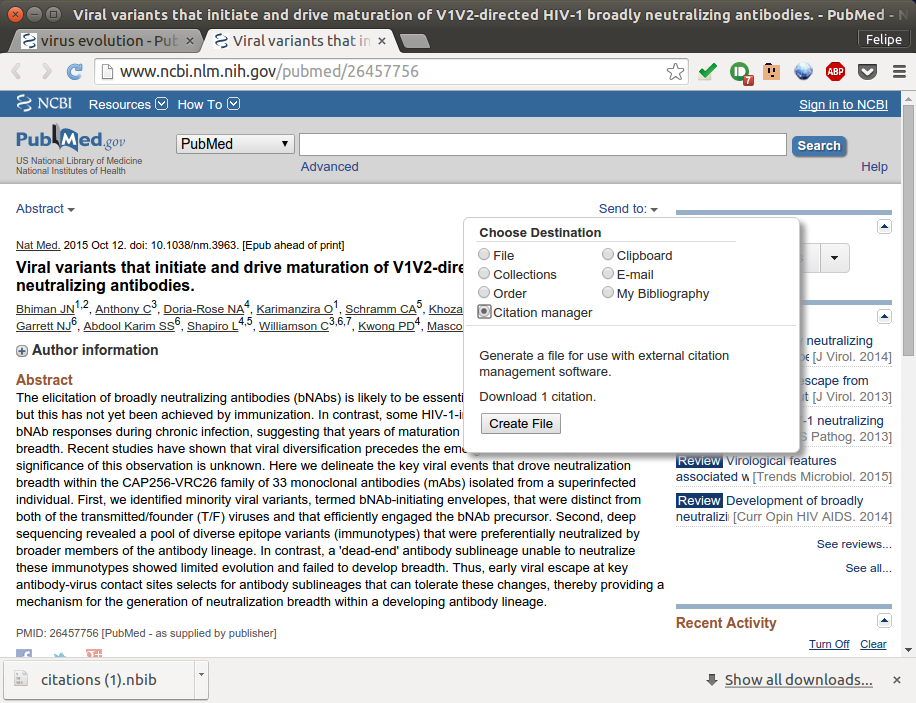
\includegraphics[height=.85\textheight]{Busca/pubmed-export1}
\end{frame}

\begin{frame}{PUBMED Exportando várias referências}
  \centering
  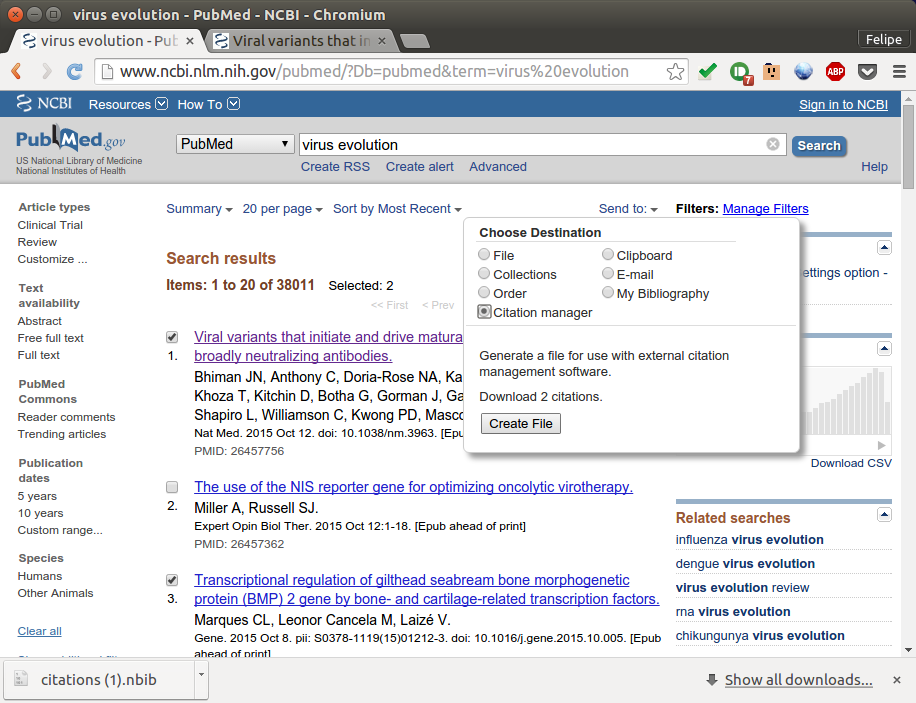
\includegraphics[height=.85\textheight]{Busca/pubmed-export2}
\end{frame}

\begin{frame}{O Paradoxo da escolha}
  \begin{block}{Pergunta}
    \footnotesize
    Nesse oceano de informações, como encontrar rapidamente uma fonte
    específica?
  \end{block}
  \pause
  \begin{block}{Resposta}
    Google
  \end{block}
\end{frame}

\subsection{Google Scholar}

\begin{frame}{Google Scholar}
  \begin{block}{Definição}
    Mecanismo de busca que acessa a base bibliográfica do Google para
    livros e artigos acadêmicos.
  \end{block}
  \begin{itemize}
    \footnotesize
  \item Escopo: A vida, o universo e tudo o mais\footnote{e obrigado
      pelo peixe}
  \item Indexa citações
  \item Facilita acesso ao PDF, caso disponível publicamente
  \item Exporta referências
  \end{itemize}
\end{frame}

\begin{frame}{Google Scholar Busca}
  \centering
  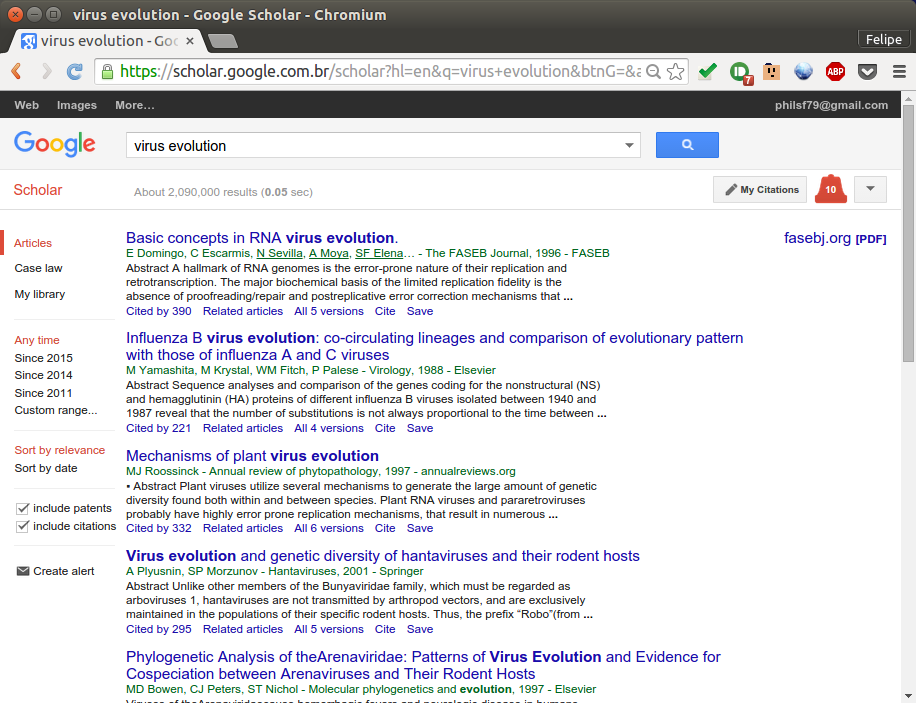
\includegraphics[height=.85\textheight]{Busca/scholar-busca1}
\end{frame}

\begin{frame}{Google Scholar Busca}
  \centering
  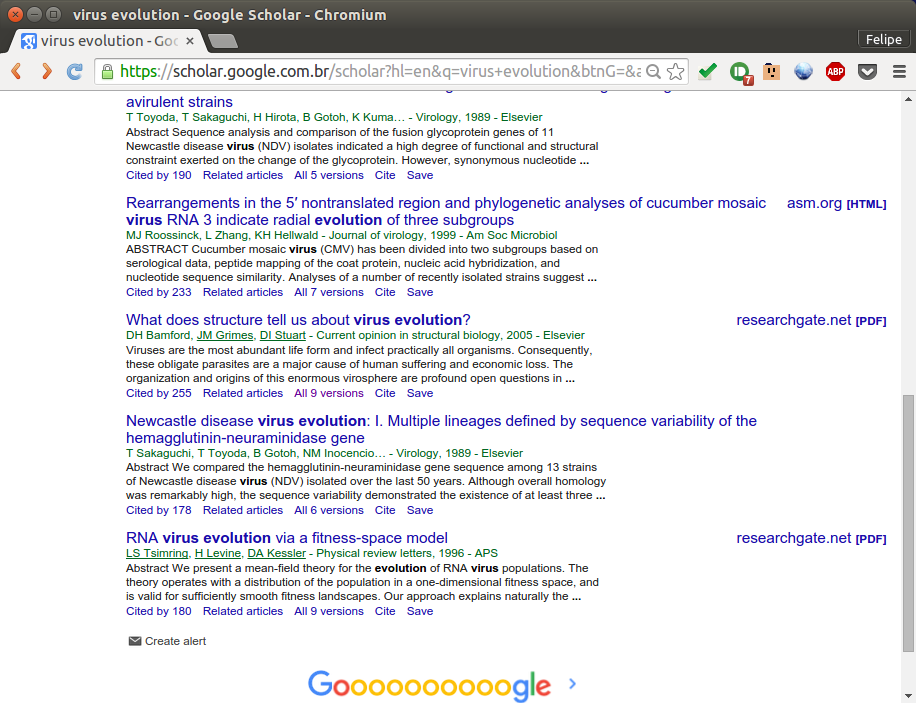
\includegraphics[height=.85\textheight]{Busca/scholar-busca2}
\end{frame}

\begin{frame}{Google Scholar Artigo}
  \begin{itemize}
    \footnotesize
  \item O Google Scholar agrega todas as versões online encontradas
    para a referência
  \item Ao acessar {\em todas as versões}, você pode consultá-las
    individualmente
  \item Caso alguém publique o conteúdo integral (PDF, HTML, DOC,
    etc), o arquivo será agregado nesta listagem
  \end{itemize}
\end{frame}

\begin{frame}{Google Scholar Artigo (todas as versões)}
  \centering
  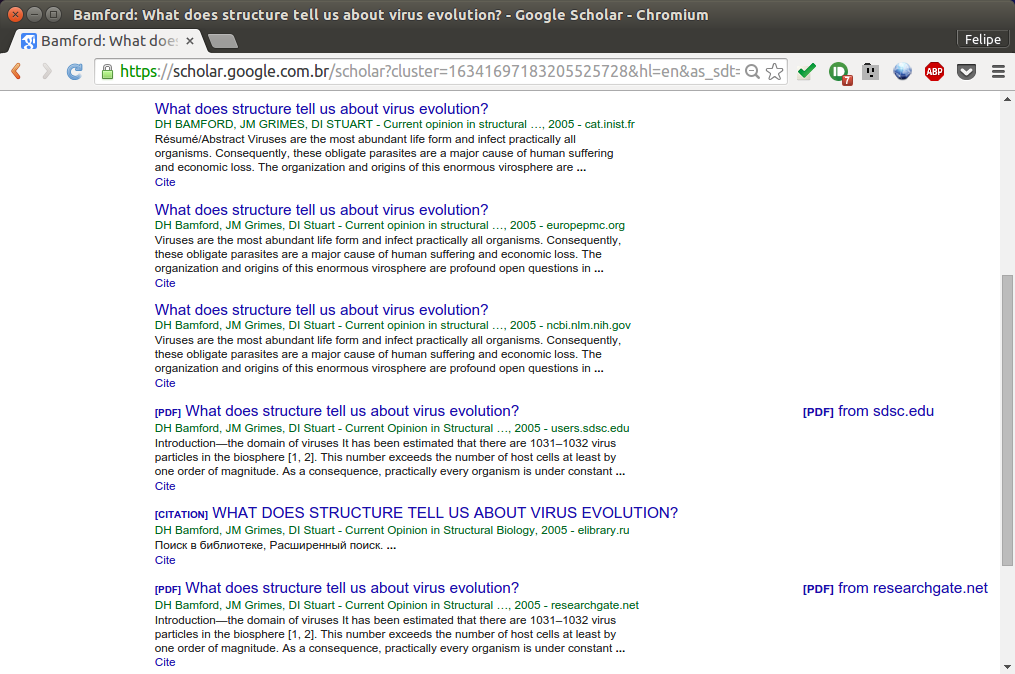
\includegraphics[height=.85\textheight]{Busca/scholar-paper}
\end{frame}

\begin{frame}{Google Scholar Exportando a Referência}
  Acessando a opção {\em citar} o Google gera a referência:
  \begin{itemize}
    \footnotesize
  \item textual, para copiar e colar (em alguns estilos de formatação)
  \item arquivo para ser importado em um gerenciador
    bibliográfico\footnote{Arquivo .RIS (RefMan): importado
      diretamente no Mendeley}
  \end{itemize}
\end{frame}

\begin{frame}{Google Scholar Exportando a Referência}
  \centering
  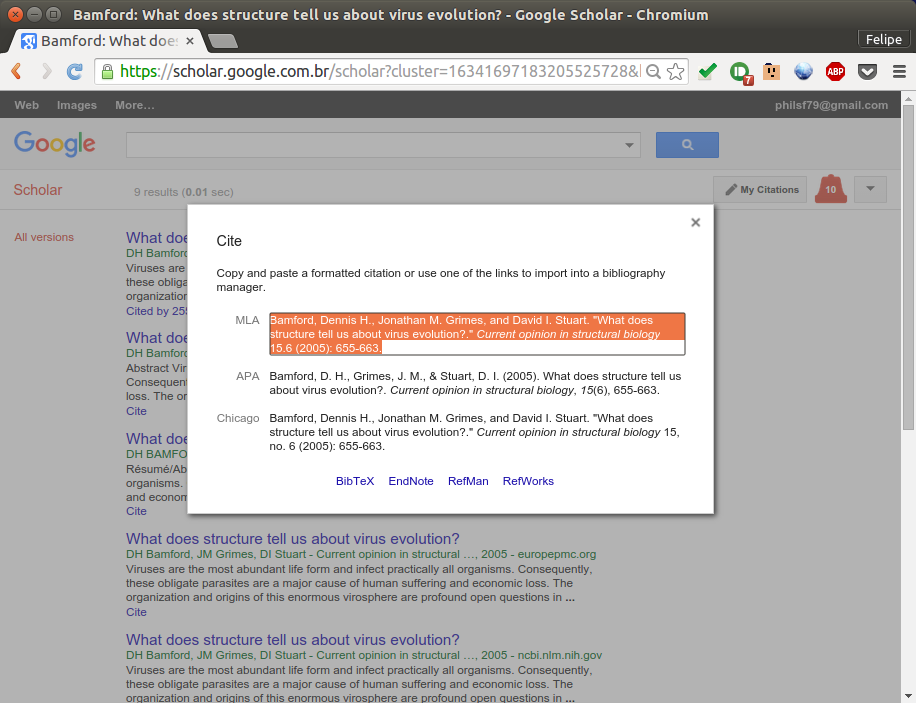
\includegraphics[height=.85\textheight]{Busca/scholar-export}
\end{frame}

\subsection{Google Books}

\begin{frame}{Google Books}
  \begin{itemize}
    \footnotesize
  \item Plataforma \alert{Google
      Books}\footnote{\url{https://books.google.com/}} (antes: Google
    Book Search e Google Print)
  \item Iniciado em 2004, digitalizou milhões de livros + OCR para
    extrair a íntegra do texto
  \item Tem 4 níveis de acesso para o acervo:
    \begin{enumerate}
      \scriptsize
    \item Full view (domínio público)
    \item Preview (\% disponível, escolha da editora)
    \item Snippet view (2--3 linhas em torno da chave de busca)
    \item No preview
    \end{enumerate}
  \end{itemize}
\end{frame}

\begin{frame}{Buscando livros no Google Books}
  Pode-se \ldots
  \begin{itemize}
    \footnotesize
  \item localizar livros buscando por:
    \begin{itemize}
      \scriptsize
    \item Metadados (autor(es) e/ou título)
    \item Trechos ou frases
    \end{itemize}
  \item consultar preview ou a íntegra (se disponível em domínio
    público)
  \item \alert{exportar} referência para \alert{importação} no
    gerenciador bibliográfico (Mendeley, Endnote, etc.)
  \end{itemize}
\end{frame}

\begin{frame}{Busca por metadados}
  \centering
  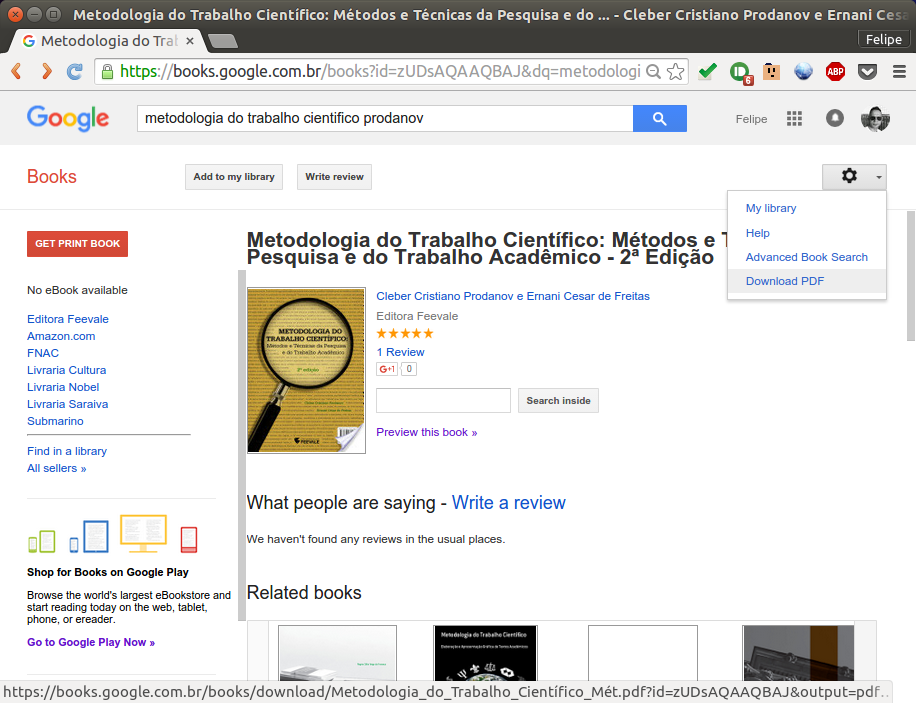
\includegraphics[height=.85\textheight]{Busca/gbooks-livro}
\end{frame}

\begin{frame}{Preview}
  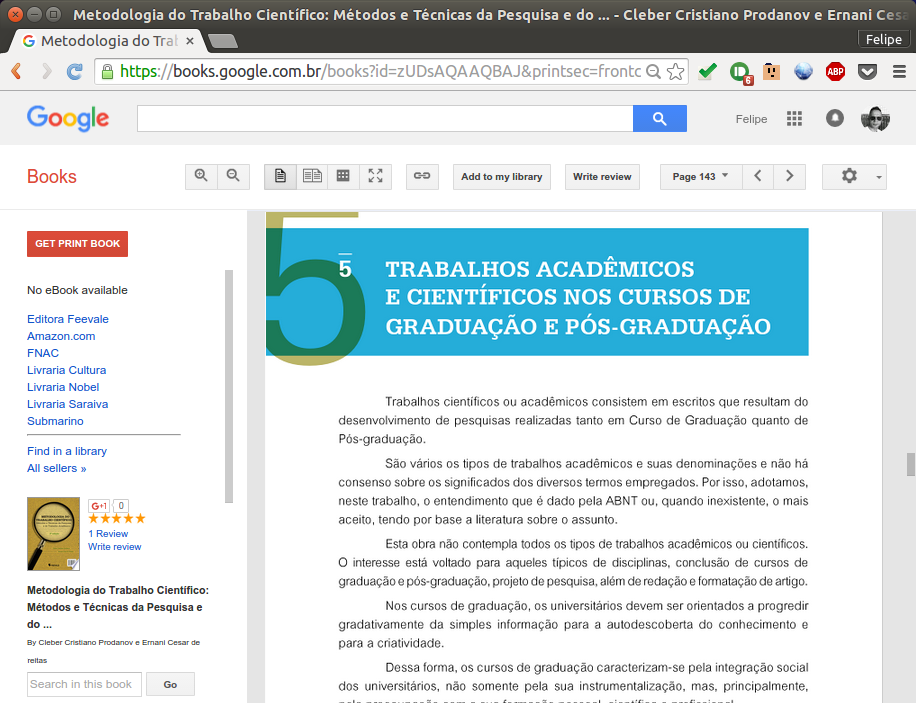
\includegraphics[height=.85\textheight]{Busca/gbooks-preview}
\end{frame}

\begin{frame}{Domínio Público}
  \centering
  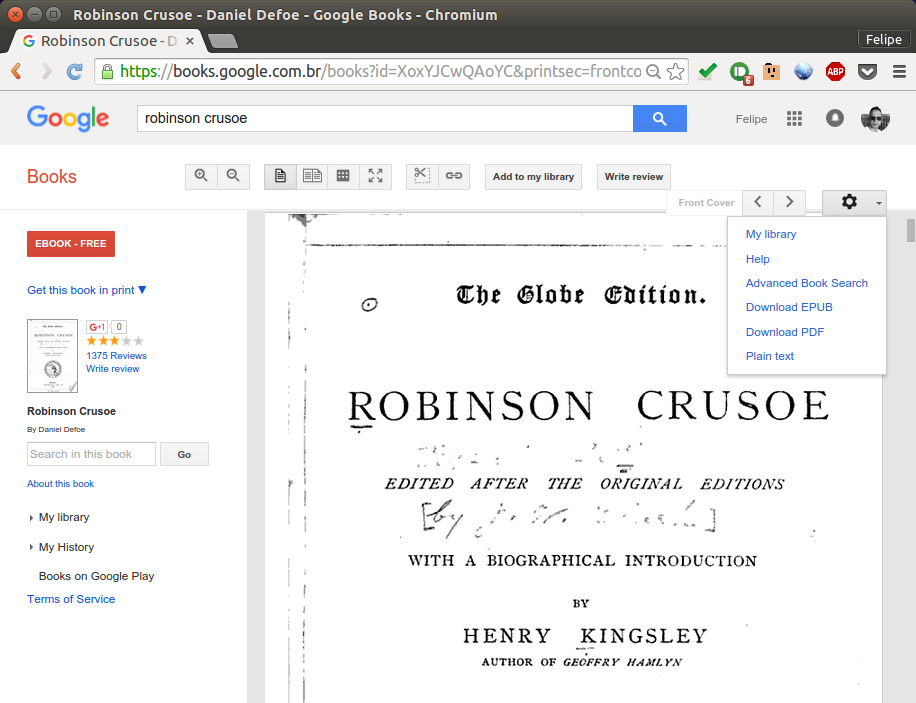
\includegraphics[height=.85\textheight]{Busca/gbooks-publicdomain}
\end{frame}

\begin{frame}{Livros acadêmicos}
  \begin{itemize}
    \footnotesize
  \item Estamos interessados em livros acadêmicos/científicos
  \item Ao fazer, e.g., uma citação direta, podemos usar o Google
    Books para:
    \begin{itemize}
      \scriptsize
    \item localizar o livro
    \item importar a referência para nosso gerenciador bibliográfico
    \end{itemize}
  \end{itemize}
  \begin{exampleblock}{Buscando a frase\ldots}
    \tiny
    \em
    ``Life depends on the ability of cells to store, retrieve, and
    translate the genetic instructions required to make and maintain a
    living organism.''
  \end{exampleblock}
\end{frame}

\begin{frame}{Busca por conteúdo}
  \centering
  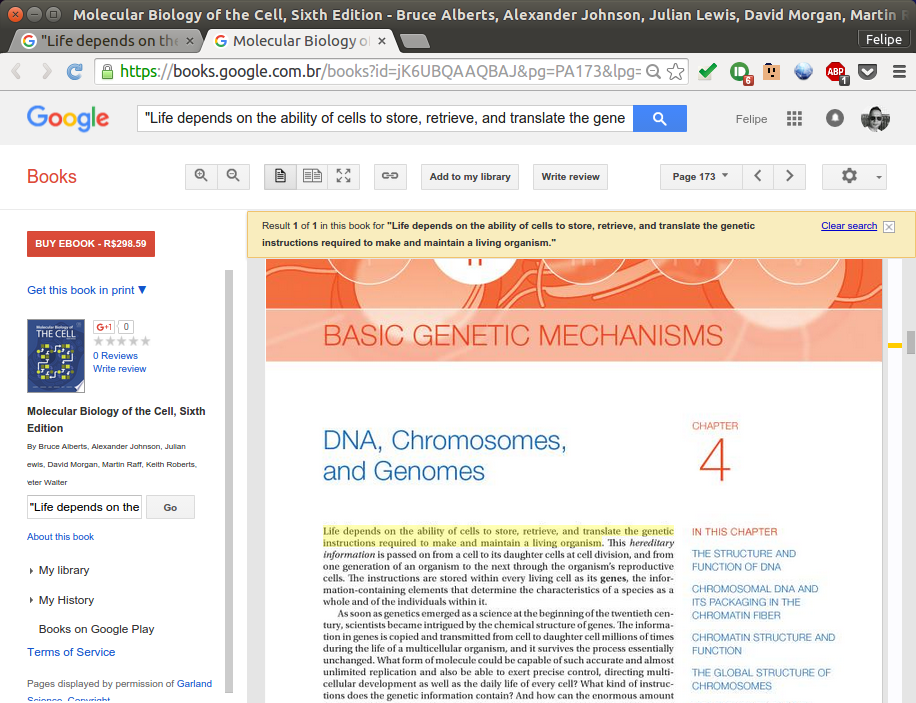
\includegraphics[height=.85\textheight]{Busca/gbooks-busca-conteudo}
\end{frame}

\begin{frame}{Importando a referência}
  \begin{itemize}
    \scriptsize
  \item Seção ``Sobre este Livro'' ({\em About this book} na coluna
    esquerda do slide anterior)
  \item Ao pé da página, temos todas as informações bibliográficas, e
    opções para baixar como arquivo
  \item A opção do arquivo .RIS (RefMan) pode ser importada pelo
    Mendeley
  \end{itemize}
\end{frame}

\begin{frame}{Sobre este livro}
  \centering
  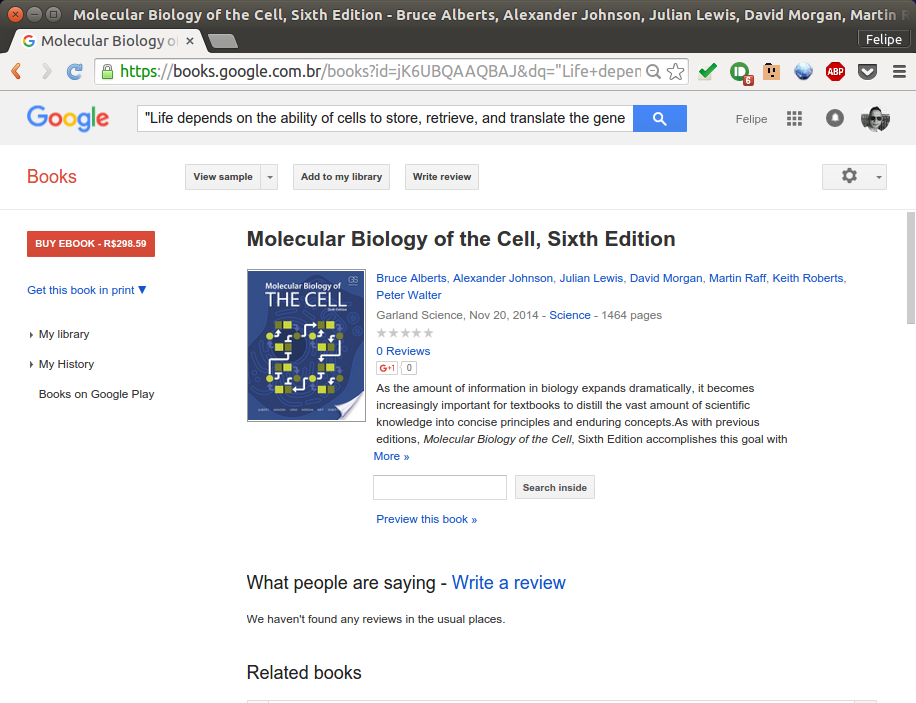
\includegraphics[height=.85\textheight]{Busca/gbooks-about1}
\end{frame}

\begin{frame}{Exportar arquivo RIS (RefMan)}
  \centering
  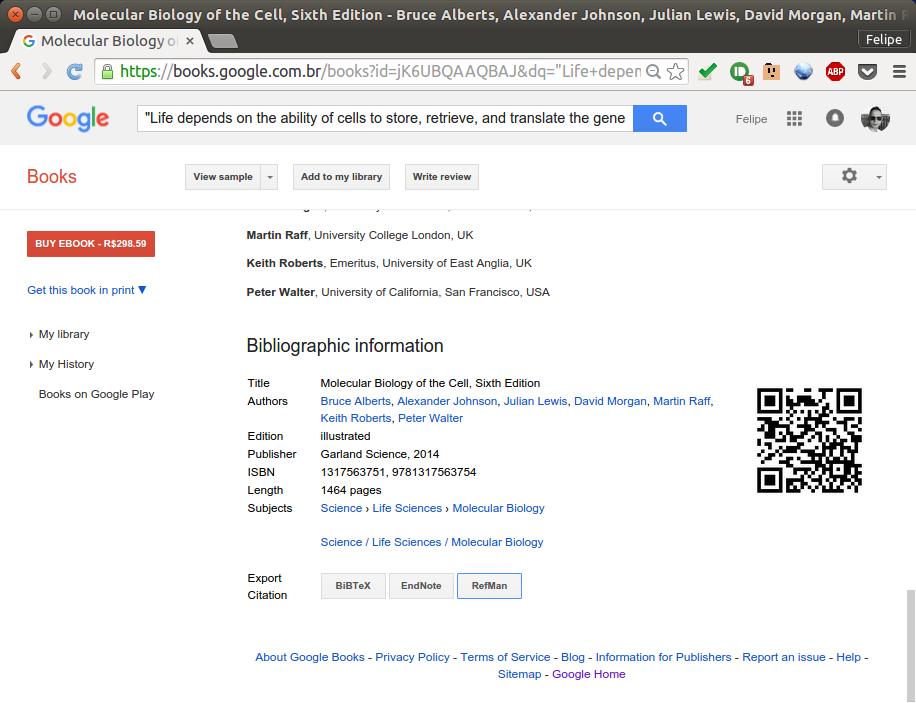
\includegraphics[height=.85\textheight]{Busca/gbooks-about2}
\end{frame}

\section{Google-fu}

\subsection{O que é}

\begin{frame}{Google-fu}
  \begin{block}{Google-fu}
    \footnotesize
    Habilidade em usar mecanismos de busca (em especial o Google) para
    localizar rapidamente informação na Internet.

    \bigskip
    Referência ao termo {\em kung fu}, cujo domínio exige muita
    dedicação.

    \bigskip
  \hfill {\tiny Fonte: \href{http://english.stackexchange.com/questions/19967/what-does-google-fu-mean}{Stack Exchange}}
  \end{block}

  \bigskip
  \begin{block}{Resumindo}
    \footnotesize
    Conjunto de técnicas ``avançadas'' usadas quando a informação
    necessária é difícil de ser localizada.
  \end{block}
\end{frame}

\subsection[{\em Advanced}]{Opções avançadas de busca}

\begin{frame}{Opções de busca}
  Podemos ampliar ou reduzir o escopo da busca \ldots
  \begin{itemize}
    \footnotesize
  \item Incluindo obrigatoriamente uma chave de busca (operador +)
  \item Excluindo uma chave de busca (operador -)
  \item Buscando uma frase exata (frase entre aspas)
  \item Combinando todas as opções acima (e outras!)
  \end{itemize}
\end{frame}

\begin{frame}{Busca básica}
  \centering
  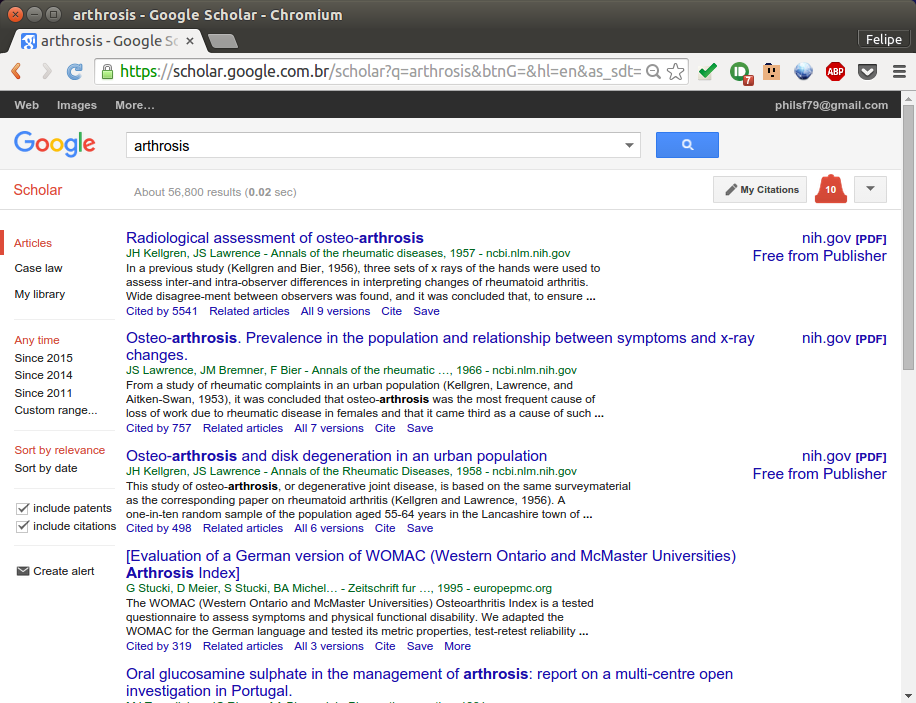
\includegraphics[height=.85\textheight]{Busca/google-fu-basico}
\end{frame}

\begin{frame}{Operador +}
  \centering
  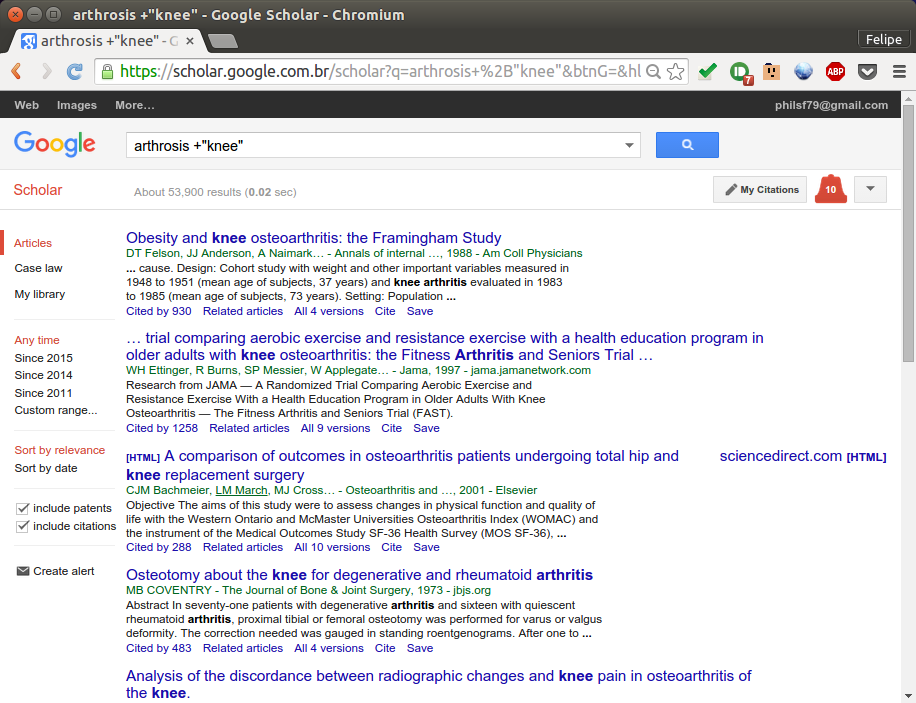
\includegraphics[height=.85\textheight]{Busca/google-fu-plus}
\end{frame}

\begin{frame}{Operador -}
  \centering
  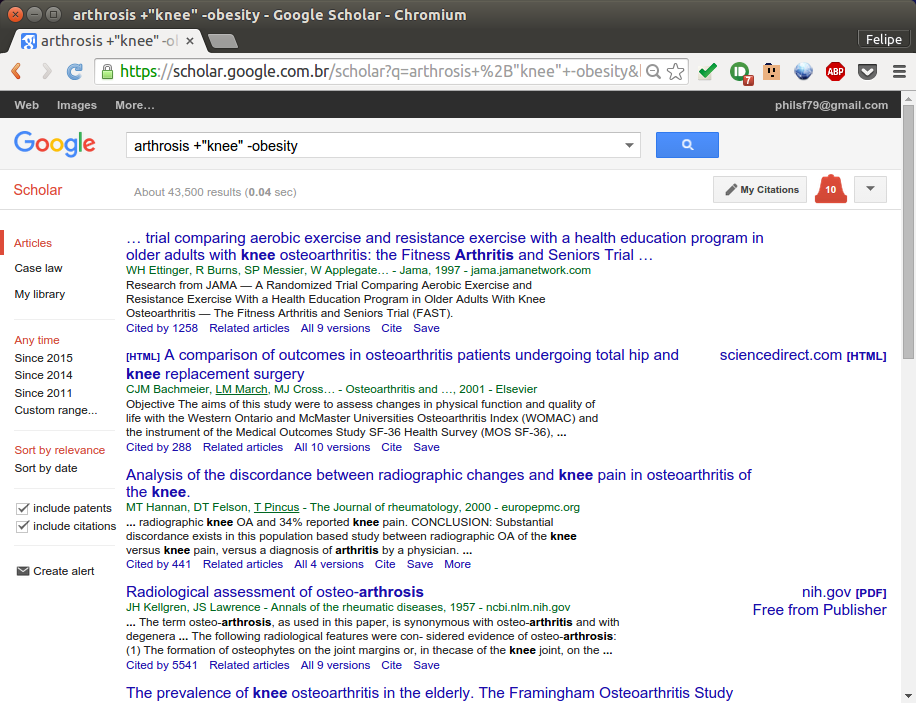
\includegraphics[height=.85\textheight]{Busca/google-fu-plusminus}
\end{frame}

\begin{frame}{Observações}
  \begin{itemize}
    \footnotesize
  \item Observe que no último exemplo, {\em obesity} foi usada sem
    aspas
  \item Isso significa que o Google não vai procurar a palavra
    \alert{exata}, mas também algumas flexões da mesma
  \end{itemize}
  \begin{exampleblock}{}
    obesity, obese, \ldots
  \end{exampleblock}
\end{frame}

\subsection[PICO]{Tópico: PICO@PUBMED}

\begin{frame}{\footnotesize Buscas por perguntas estruturadas no PUBMED}
  \begin{itemize}
    \footnotesize
  \item PUBMED: possui interface de busca estruturada
    \bigskip
  \item Estrutura: pergunta PICO
    \bigskip
  \item Avaliadas 2 interfaces x interface padrão de busca (2007)
  \end{itemize}

  \vfill
  \tiny
  \hfill \href{https://doi.org/10.1186/1472-6947-7-16}{SCHARDT et al, 2007}
\end{frame}

\begin{frame}{\footnotesize Buscas por perguntas estruturadas no PUBMED}
  \begin{exampleblock}{Interfaces PICO@PUBMED}
    \centering
    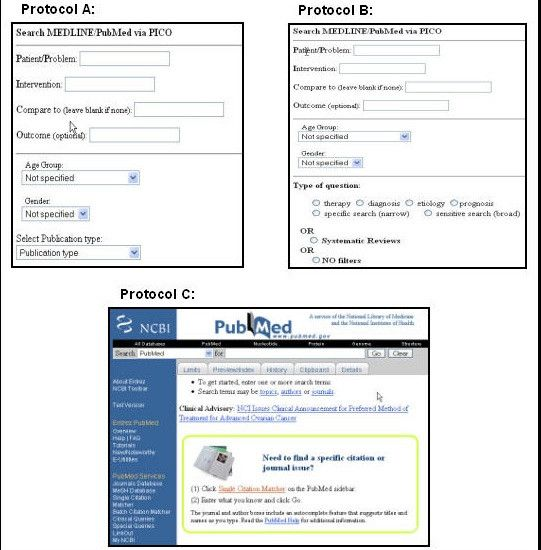
\includegraphics[height=.8\textheight]{Busca/pubmed-pico}
  \end{exampleblock}

  \vfill
  \tiny
  \hfill \href{https://doi.org/10.1186/1472-6947-7-16}{SCHARDT et al, 2007}
\end{frame}

\begin{frame}{\footnotesize Principais características do estudo}
  \begin{itemize}
    \footnotesize
  \item {\bf Objetivo:} Comparação das duas interfaces PICO ({\tiny em relação ao padrão})
    \bigskip
  \item {\bf Desfecho primário:} precisão ({\tiny proporção de citações {\em relevantes} em relação ao total})
    \bigskip
  \item {\bf Resultado:} maior precisão em ambos os PICO ({\tiny que na interface padrão})
    \bigskip
  \item {\bf Conclusão:}
    \begin{itemize}
      \scriptsize
    \item Amostra pequena para observar significância estatística
    \item Recomendação de buscar por PICO
    \end{itemize}
    \bigskip
  \item {\bf Obs:} links para as interfaces nas refs do paper
  \end{itemize}

  \vfill
  \tiny
  \hfill \href{https://doi.org/10.1186/1472-6947-7-16}{SCHARDT et al, 2007}
\end{frame}

\section{Outras fontes}

\subsection{Deep Web}

\subsubsection{Papers}

\begin{frame}{Como baixar artigos pagos}
Já vimos as principais maneiras de se obter artigos
  \begin{itemize}
    \footnotesize
  \item Acessar de uma instituição que assina a revista/editora
  \item Portal CAPES Periódicos
  \item Google Scholar
  \end{itemize}
\end{frame}

\begin{frame}{Vejamos outras}
  \begin{itemize}
    \footnotesize
  \item Página profissional do autor/lab
  \item Redes sociais acadêmicas (autor)
    \begin{itemize}
    \item Research Gate - \url{www.researchgate.net}
    \item Academia.edu - \url{www.academia.edu}
    \end{itemize}
  \item E-mail para o autor correspondente
  \item etc...
  % \item SCIHUB - \url{http://sci-hub.cc/}
  \end{itemize}
  \begin{block}{Obs}
    \begin{itemize}
    \footnotesize
    \item O Scholar indexa PDFs das fontes acima
    \item ... nem sempre o índice do Google está atualizado
    \item $\Rightarrow$ procurar manualmente
    \end{itemize}
  \end{block}
\end{frame}

\begin{frame}{Exemplo - artigo}
  \begin{center}
    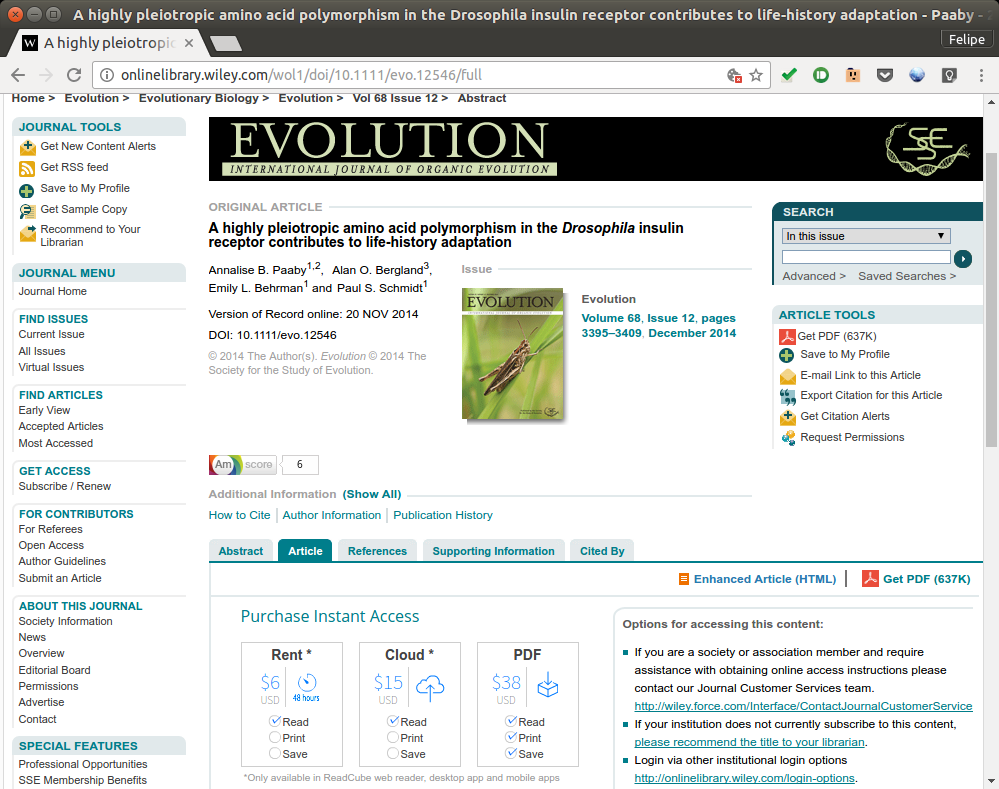
\includegraphics[height=.9\textheight]{Busca/petrov1}
  \end{center}
\end{frame}

\begin{frame}{Exemplo - página do autor/lab}
  \begin{center}
    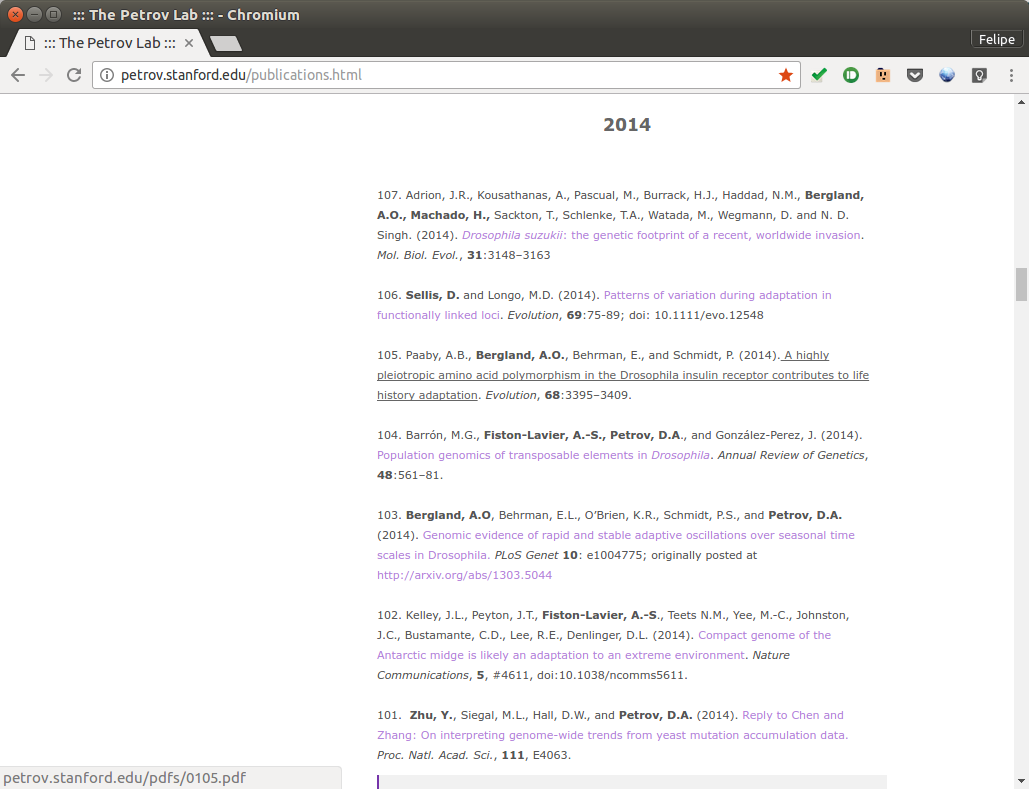
\includegraphics[height=.9\textheight]{Busca/petrov2}
  \end{center}
\end{frame}

\begin{frame}{O Sci-Hub}
  \begin{itemize}
    \footnotesize
  \item Artigos pagos estão disponíveis para assinantes
  \item O mecanismo de verificação pode ser ``burlado'' usando um
    endereço (de internet) de uma instituição assinante
  \item O SCIHUB automatiza esse procedimento
  \end{itemize}
\end{frame}

\begin{frame}{O Sci-Hub: Filosofia Hacker}
  \begin{itemize}
    \footnotesize
  \item Hackers acreditam que {\em a informação deve ser livre}, para
    benefício amplo da sociedade (\alert{especialmente} se financiados
    com verba pública)
  \item Filosofia Open-Source $\Rightarrow$ artigos Open-Access
  \item Visão: ``{\em coletar todos os papers de pesquisa já
      publicados e disponibilizá-los gratuitamente}''.
  \item Vários espelhos ao redor do mundo, ocasionalmente saem do ar e
    são substituídos
  \end{itemize}

  \tiny
  \hfill Fonte: \url{https://torrentfreak.com/sci-hub-tears-down-academias-illegal-copyright-paywalls-150627/}
\end{frame}

\begin{frame}{Usando o Sci-hub}
  \begin{itemize}
    \footnotesize
  \item Localize o artigo pago no site da editora
  \item Copie o endereço completo do artigo
  \item Cole o endereço na busca do Sci-Hub (e torça para estar
    disponível no acervo)
  \end{itemize}
  \begin{block}{Endereço (atualizado em 2016)}
    SCIHUB - \url{http://sci-hub.cc/}
  \end{block}
\end{frame}

\begin{frame}{Usando o Sci-hub}
  \centering
  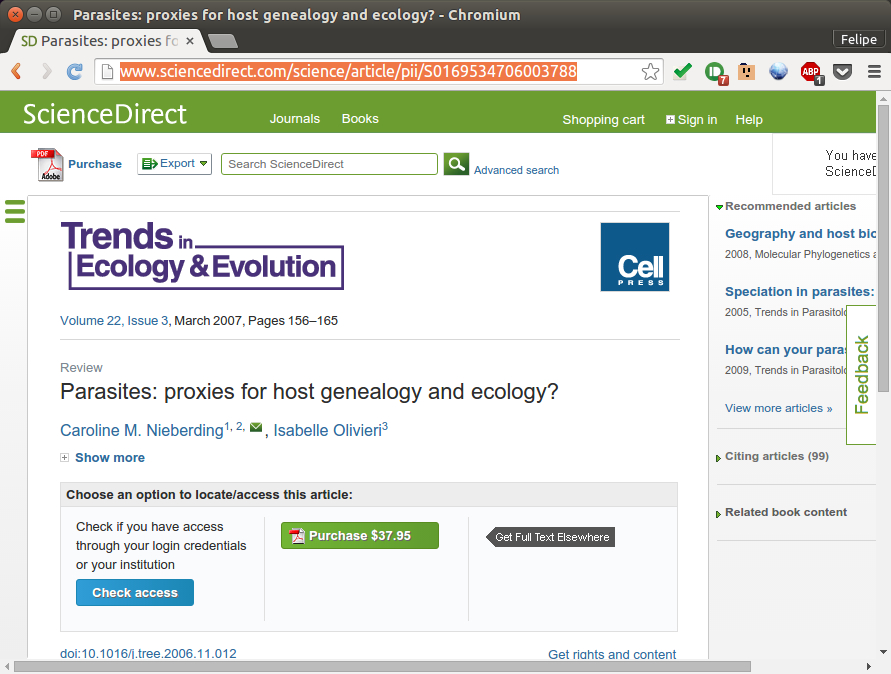
\includegraphics[height=.85\textheight]{Busca/scihub-busca1}
\end{frame}

\begin{frame}{Usando o Sci-hub}
  \centering
  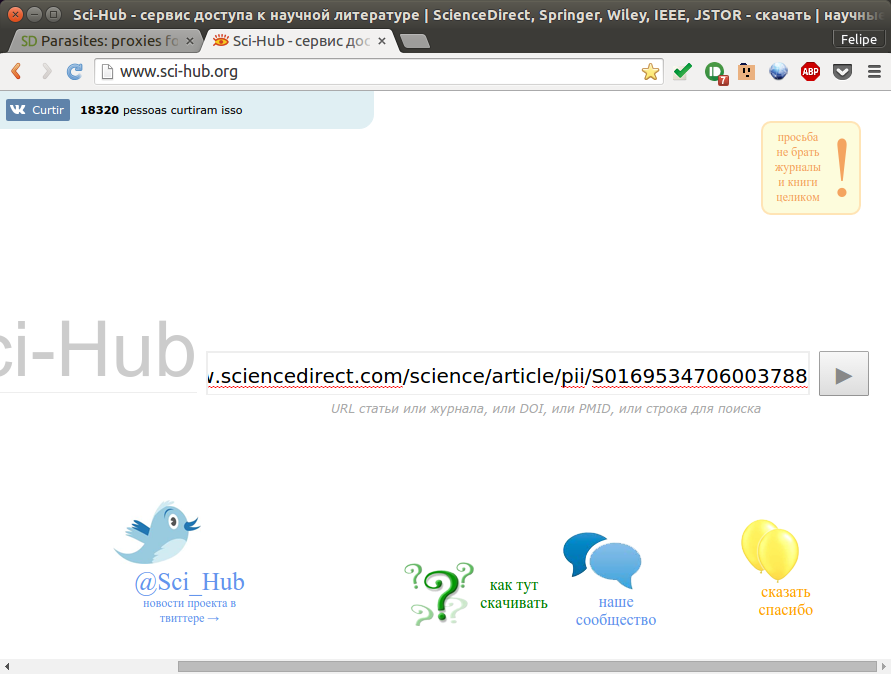
\includegraphics[height=.85\textheight]{Busca/scihub-busca2}
\end{frame}

\begin{frame}{Usando o Sci-hub}
  \centering
  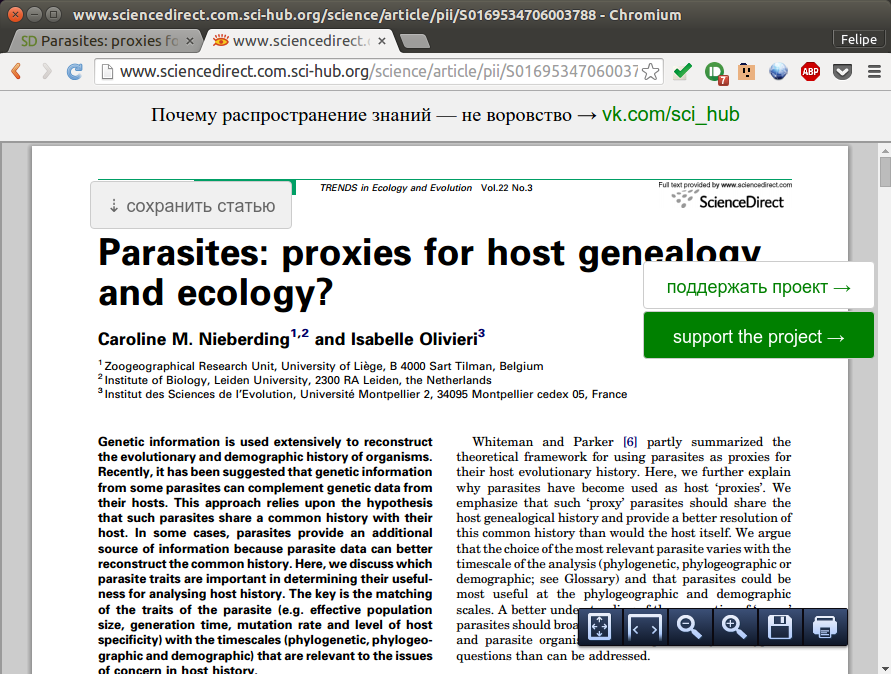
\includegraphics[height=.85\textheight]{Busca/scihub-busca3}
\end{frame}

\subsubsection{Livros}

\begin{frame}{Libgen: Library Genesis}
  \begin{itemize}
    \footnotesize
  \item Semelhante ao sci-hub, mas especializado em e-books
  \item Link (hoje oculto) localiza livros científicos:
    \alert{/scimag}
  \item Endereço original: \url{http://libgen.io/scimag} (inativo)
  \item Espelho funcional (hoje): \url{http://gen.lib.rus.ec/}\footnote{\url{https://sites.google.com/site/themetalibrary/library-genesis}}
  \end{itemize}
\end{frame}

\begin{frame}{Libgen}
  \centering
  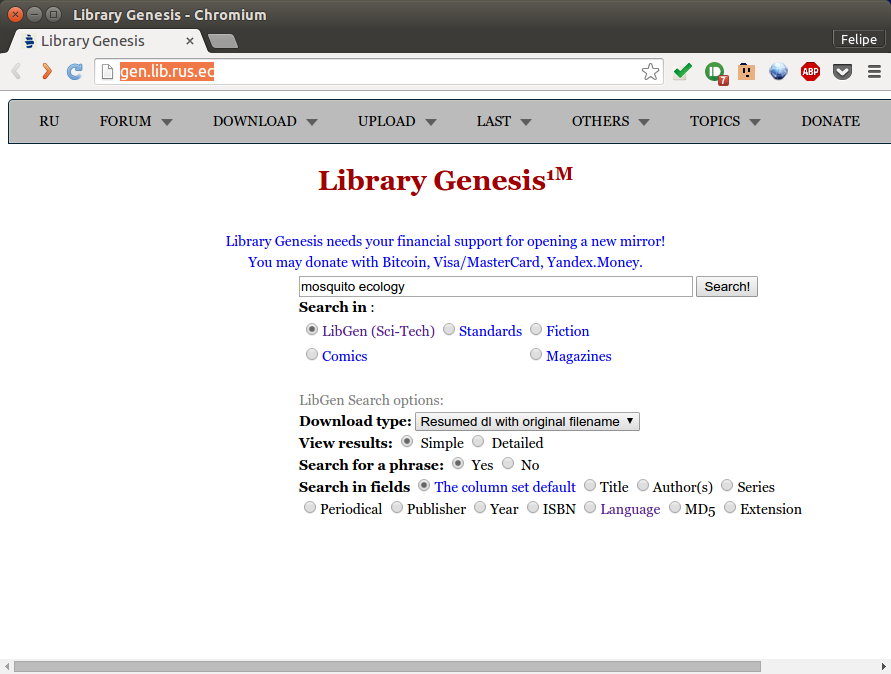
\includegraphics[height=.85\textheight]{Busca/libgen-busca1}
\end{frame}

\begin{frame}{Libgen}
  \centering
  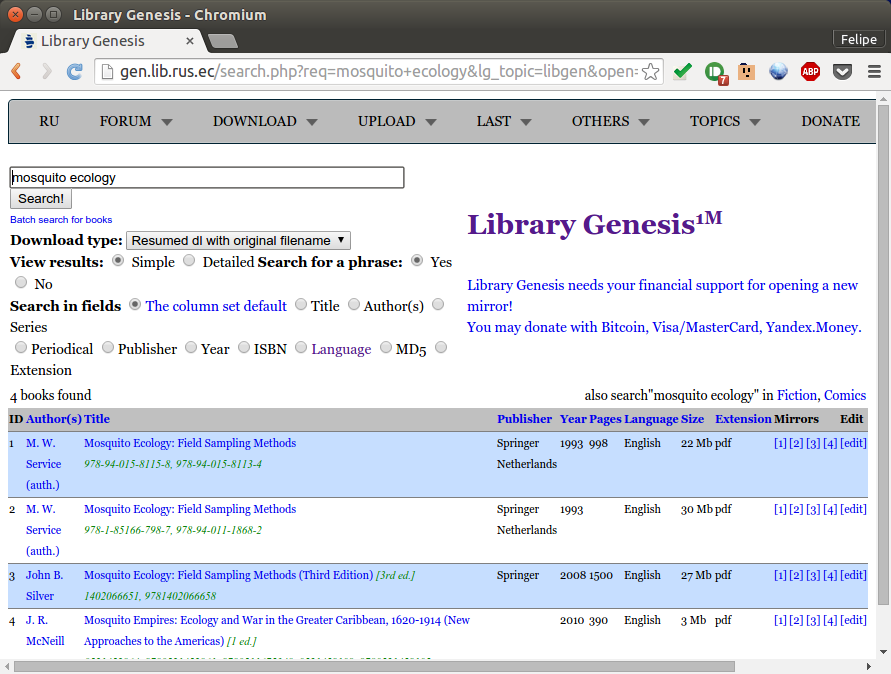
\includegraphics[height=.85\textheight]{Busca/libgen-busca2}
\end{frame}

\section{Aprofundamento}

\subsection{Aprofundamento}

\begin{frame}{Aprofundamento}
  \begin{block}{Leitura obrigatória}
    \scriptsize
    \href{https://doi.org/10.1186/1472-6947-7-16}{SCHARDT, Connie et al. Utilization of the PICO framework to improve searching PubMed for clinical questions. {\bf BMC medical informatics and decision making}, v. 7, n. 1, p. 16, 2007.}
  \end{block}
  \begin{block}{Leitura recomendada}
  \end{block}
\end{frame}

\end{document}
